\documentclass[11pt]{article}
	\usepackage[T1]{fontenc}
    % Nicer default font (+ math font) than Computer Modern for most use cases
    % \usepackage{mathpazo}

    % Basic figure setup, for now with no caption control since it's done
    % automatically by Pandoc (which extracts ![](path) syntax from Markdown).
    \usepackage{graphics}
    % We will generate all images so they have a width \maxwidth. This means
    % that they will get their normal width if they fit onto the page, but
    % are scaled down if they would overflow the margins.
    \makeatletter
    \def\maxwidth{\ifdim\Gin@nat@width>\linewidth\linewidth
    \else\Gin@nat@width\fi}
    \makeatother
    \let\Oldincludegraphics\includegraphics
    % Set max figure width to be 80% of text width, for now hardcoded.
    \renewcommand{\includegraphics}[1]{\Oldincludegraphics[width=.8\maxwidth]{#1}}
    % Ensure that by default, figures have no caption (until we provide a
    % proper Figure object with a Caption API and a way to capture that
    % in the conversion process - todo).
    \usepackage[center,bf]{caption}
    % \DeclareCaptionLabelFormat{nolabel}{}
    % \captionsetup{labelformat=nolabel}

    \usepackage{adjustbox} % Used to constrain images to a maximum size 
    \usepackage{xcolor} % Allow colors to be defined
    \usepackage{enumerate} % Needed for markdown enumerations to work
    \usepackage{geometry} % Used to adjust the document margins
    \usepackage{amsmath} % Equations
    \usepackage{amssymb} % Equations
    \usepackage{textcomp} % defines textquotesingle
    % Hack from http://tex.stackexchange.com/a/47451/13684:
    \AtBeginDocument{%
        \def\PYZsq{\textquotesingle}% Upright quotes in Pygmentized code
    }
    \usepackage{upquote} % Upright quotes for verbatim code
    \usepackage{eurosym} % defines \euro
    \usepackage[mathletters]{ucs} % Extended unicode (utf-8) support
    \usepackage[utf8x]{inputenc} % Allow utf-8 characters in the tex document
    \usepackage{fancyvrb} % verbatim replacement that allows latex
    \usepackage{grffile} % extends the file name processing of package graphics 
                         % to support a larger range 
    % The hyperref package gives us a pdf with properly built
    % internal navigation ('pdf bookmarks' for the table of contents,
    % internal cross-reference links, web links for URLs, etc.)
    \usepackage{hyperref}
    \usepackage{longtable} % longtable support required by pandoc >1.10
    \usepackage{booktabs}  % table support for pandoc > 1.12.2
    \usepackage[inline]{enumitem} % IRkernel/repr support (it uses the enumerate* environment)
    \usepackage[normalem]{ulem} % ulem is needed to support strikethroughs (\sout)
                                % normalem makes italics be italics, not underlines
   	\usepackage[]{authblk}
   	\usepackage{cite}
    \usepackage{graphicx}
    \usepackage{hyperref}
    \usepackage{amsmath}
    \usepackage{amsthm}
    \usepackage{amssymb}
    \usepackage{bm}
    \usepackage{bbm}
    \usepackage{algorithmicx}
    \usepackage{algorithm}
    \usepackage{algpseudocode}
    \usepackage{array}
    \usepackage{booktabs}
    \usepackage{multirow}
    \usepackage{makecell}
    \usepackage{color}
    \usepackage{tabularx,ragged2e,booktabs,caption}
    \usepackage{verbatim}
   	\makeatletter
    \def\@maketitle{%
    \newpage
      \null
      \vskip 2em%
      \begin{center}%
      \let \footnote \thanks
        {\Large\bfseries \@title \par}%
        \vskip 1.5em%
        {\normalsize
          \lineskip .5em%
          \begin{tabular}[t]{c}%
            \@author
          \end{tabular}\par}%
        \vskip 1em%
        {\normalsize \@date}%
      \end{center}%
      \par
      \vskip 1.5em}
    \makeatother


\newtheorem{theorem}{Theorem}






\title{EE 219 Project 1 Classification Analysis on Textual Data}
\author{Zhilai~Shen, Yufei~Hu, Zheang~Huai, and Tianyi~Liu
}


\date{\today}


\begin{document}
\maketitle

\begin{comment}
\section{A brief tutorial on how to use this template}
\Large\textcolor{red}{\bf{Please remove the tutorial section in the final manuscript\\ by commenting, i.e. $\%(something)$}}


\subsection{Figures}
Figure insertion is shown in Fig \ref{example_fig}.
\begin{figure}[h]
\centering
\scalebox{0.7}{\includegraphics{Figures/spectrum_bar.pdf}}
\caption{An example of figure insertion}
\label{example_fig}
\end{figure}

\subsection{Equations}
An example of equations is given as follows.
\begin{theorem}
Let $a$, $b$, $c$ denote the sides of a triangle, respectively. If $a\perp b$, the pythagoras theorem is given as follows.
\begin{align}
c^2 = a^2 + b^2
\end{align}
\end{theorem}

\subsection{Tables}
An example of tables is shown in Table \ref{example_table}.
\renewcommand\arraystretch{1.1}
\begin{table}[h]
\center
\caption{Standard CRC Codes versus Optimal CRC Codes for Convolutional Code $G=(561~753)$ with $n=504$ Bits}
\scalebox{0.9}{
\begin{tabular}{r|c|c|cccccc}
\hline
\multirow{2}{*}{Name} & \multirow{2}{*}{Gen. Poly.} & \multicolumn{7}{c}{Undetected Error Distance Spectrum} \\
\cline{3-9}
 & & $d$ & 16 & 18 & 20 & 22 & 24 & 26 \\\hline\hline
Standard-8 & \multicolumn{1}{l}{0x19B} & & 983 & 4387 & 19909 & 105000 & 672724 & 3972970\\
Optimal-8 & \multicolumn{1}{l}{0x19D} & & 0 & 979 & 22349 & 111304 & 686314 & 3830340\\\hline
Standard-12 & \multicolumn{1}{l}{0x180F} & & 0 & 0 & 969 & 5815 & 42893 & 245211 \\
Optimal-12 & \multicolumn{1}{l}{0x108B} & & 0 & 0 & 0 & 4793 & 45795 & 246729\\\hline
Standard-16 & \multicolumn{1}{l}{0x11021} & & 0 & 0 & 484 & 0 & 1765 & 14752\\
Optimal-16 & \multicolumn{1}{l}{0x1F8FD} & & 0 & 0 & 0 & 0 & 0 & 13240\\\hline
\end{tabular}}
\label{example_table}
\end{table}

 \end{comment}

\section{Getting familiar with the dataset}

\textbf{Question 1:}

After loading the 20 categories from trianing set, we are able to view the historgram which shows the distribution of number of training documents in these 20 categories. The graph is shown as following, and from the historgram, the number of training documents in each categories is almost the same.

\begin{figure}[h]
\centering
\scalebox{0.8}{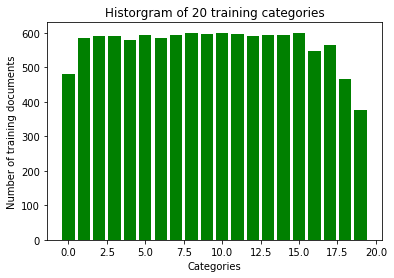
\includegraphics{Figures/Q1.png}}
\caption{Historgram of 20 Categories}
\label{fig:Q1}
\end{figure}


\section{Binary Classification}

\subsection{Feature Extraction}

\textbf{Question 2:}

Since we are only interested in 8 categories, while loading the data, "category" is a list containing these eight targeted categories. The stopwords are set to "english" as required, and one regular expression is used to get rid of numeric terms. Min\_df is set to be 3. The lemmatization and pos\_tag are also applied to combined term words with same root word. 

\bigbreak

After the above process, the shape of the TF-IDF matrices of the train subsets is $(4732, 16292)$ and that of rge test subsets is $(3150, 16292)$.


\subsection{Dimensionality Reduction}

\textbf{Question 3:}

Once we have the TF-IDF matrix, dimension reduction needs to be performed on the TF-IDF matrices by 1) LSI and 2) NMF. \textit{TruncatedSVD()} and \textit{NMF} modules in \textit{scikit learn} are used and number of components is set to be 50. Data is then loaded for further use.

\bigbreak

The square of Frobenius distance between original training data and reconstructed training data using LSI and NMF are 4103.50 and 4143.26 respectively. LSI seems to be slightly better than NMF for performing dimensionality reduction in this case.

\bigbreak

To explain the possible reason behind this observation, differences between LSI and NMF have to be analyzed. NMF split a matrix R into the product of two matrices W and H. Here R is usually very sparse. In such cases NMF works better as the missing-values assumption is inbuilt to the algorithm. In case of LSI, it does not assume anything about sparsity of the original data. And LSI usually works better when the input matrix is not too sparse.  LSI results are more deterministic compared to that of NMF. In our case, the possible reason for the observation might be due to the TF-IDF matrix is not too sparse.

\subsection{Classification Algorithms}

\subsubsection{SVM}

\textbf{Question 4:}

\begin{figure}[h]
\centering
\scalebox{0.8}{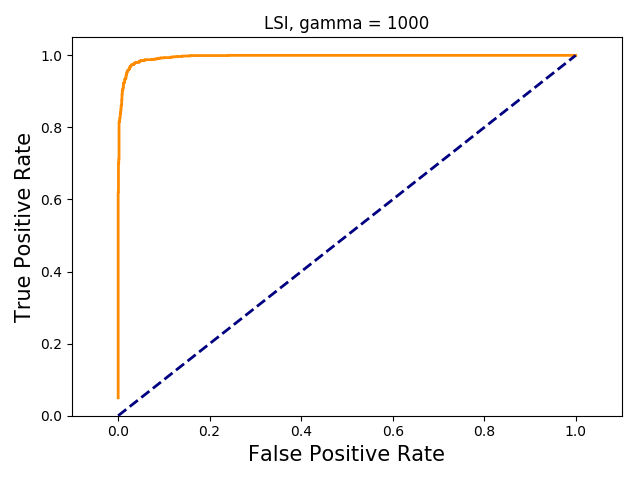
\includegraphics{Figures/Q4_1.png}}
\caption{ROC for hard margin SVM (LSI, $\gamma$=1000)}
\label{fig:Q4_1}
\end{figure}

\begin{table}[h]
\center
\caption{Performances for hard margin SVM (LSI, $\gamma$=1000)}
\scalebox{0.9}{
\begin{tabular}{r|c}
\hline
Accuracy & 0.9714 \\\hline
Recall & 0.9792 \\\hline
Precision & 0.9647 \\\hline
F1 Score & 0.9719\\\hline
\end{tabular}}
\label{tab:Q4_1_1}
\end{table}

\begin{table}[h]
\center
\caption{Performances for hard margin SVM (LSI, $\gamma$=1000)}
\scalebox{0.9}{
\begin{tabular}{r|c|c}
\hline
 & Computer tech (predict) & Recreation (predict) \\\hline
Computer tech (true) & 1503 & 57 \\\hline
Recreation (true) & 33 & 1557 \\\hline
\end{tabular}}
\label{tab:Q4_1_2}
\end{table}

\begin{figure}[h]
\centering
\scalebox{0.8}{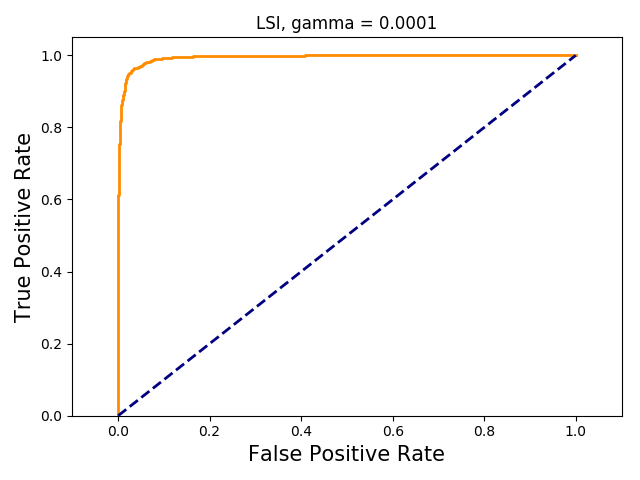
\includegraphics{Figures/Q4_2.png}}
\caption{ROC for soft margin SVM (LSI, $\gamma$=0.0001)}
\label{fig:Q4_2}
\end{figure}

\begin{table}[h]
\center
\caption{Performances for soft margin SVM (LSI, $\gamma$=0.0001)}
\scalebox{0.9}{
\begin{tabular}{r|c}
\hline
Accuracy & 0.5048 \\\hline
Recall & 1.0000 \\\hline
Precision & 0.5048 \\\hline
F1 Score & 0.6709\\\hline
\end{tabular}}
\label{tab:Q4_2_1}
\end{table}

\begin{table}[h]
\center
\caption{Performances for soft margin SVM (LSI, $\gamma$=0.0001)}
\scalebox{0.9}{
\begin{tabular}{r|c|c}
\hline
 & Computer tech (predict) & Recreation (predict) \\\hline
Computer tech (true) & 0 & 1560 \\\hline
Recreation (true) & 0 & 1590 \\\hline
\end{tabular}}
\label{tab:Q4_2_2}
\end{table}

A hard margin and a soft margin SVM classifiers using linear kernel are trained based on training data from LSI. Their ROC curve are shown in \ref{fig:Q4_1} and \ref{fig:Q4_2} respectively. Other performances can be found in \ref{tab:Q4_1_1}, \ref{tab:Q4_1_2}, \ref{tab:Q4_2_1}, \ref{tab:Q4_2_2}.

\bigbreak

Based on the results, we have observed that hard margin classifier performs much better than soft margin classifier in terms of all metrics. It appears that all instances in the test set are predicted to be recreation-related when using the soft margin classifier. Typically, a hard margin SVM works better when the data is more linearly separable. Also, a too high penalty parameter C could lead to overfitting problem while a too low C could cause underfitting problem. In our case, the instances are more difficult to fit considering their scales and dimensions (50 is still quite large to a classification problem), therefore we need an SVM classifier with a higher C to deal with such dataset. This is the reason why hard margin SVM classifier outperforms soft margin SVM classifier.

\bigbreak

Soft margin SVM classifier may have underfitted based on its confusion matrix listed in \ref{tab:Q4_2_2}. Therefore, its ROC curve looks not so good which is also shown in \ref{fig:Q4_2}. There is a sharper turning at the top-left corner in \ref{fig:Q4_2} comparing to \ref{fig:Q4_1}, the reason is because soft margin SVM classifier either has a high true positive rate with a low false positive rate or a low true positive rate with a high false positive rate. There does not exist a sweetspot that makes both true positive rate and false positive rate reach a good balance. Thus, no conflict is found between ROC and other metrics for the soft margin SVM classifier.

\bigbreak

\begin{figure}[h]
\centering
\scalebox{0.8}{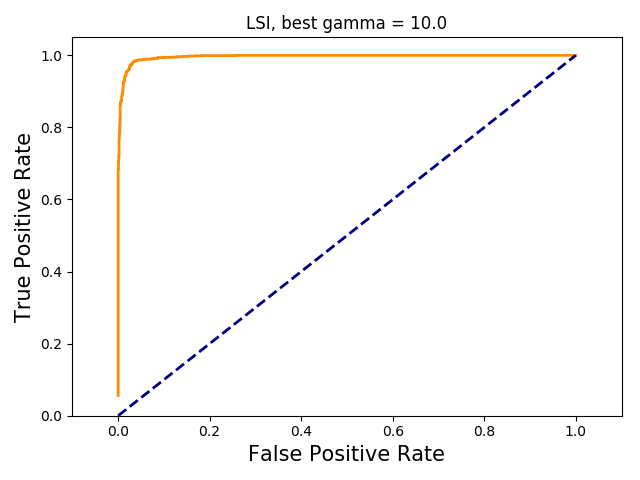
\includegraphics{Figures/Q4_3.png}}
\caption{ROC for best SVM (LSI, $\gamma$=10)}
\label{fig:Q4_3}
\end{figure}

\begin{table}[h]
\center
\caption{Performances for best SVM (LSI, $\gamma$=10)}
\scalebox{0.9}{
\begin{tabular}{r|c}
\hline
Accuracy & 0.9740 \\\hline
Recall & 0.9805 \\\hline
Precision & 0.9683 \\\hline
F1 Score & 0.9744\\\hline
\end{tabular}}
\label{tab:Q4_3_1}
\end{table}

\begin{table}[h]
\center
\caption{Performances for best SVM (LSI, $\gamma$=10)}
\scalebox{0.9}{
\begin{tabular}{r|c|c}
\hline
 & Computer tech (predict) & Recreation (predict) \\\hline
Computer tech (true) & 1509 & 51 \\\hline
Recreation (true) & 31 & 1559 \\\hline
\end{tabular}}
\label{tab:Q4_3_2}
\end{table}

After applying 5-fold cross validation, we found that the best value of the penalty parameter $\gamma$ for linear SVM classifier is 10. We then perform same evaluation. ROC curve, confusion matrix and other metrics can be found in \ref{fig:Q4_3}, \ref{tab:Q4_3_1} and \ref{tab:Q4_3_2}.


\subsubsection{Logistic Regression}

\textbf{Question 5:}

We trained a logistic classifier without regularization. The ROC curve is shown in Figure \ref {fig:LR1}. The other classification measure results are presented in Table \ref{tab:LR1}.

\bigbreak


\begin{figure}[h]
\centering
\scalebox{0.9}{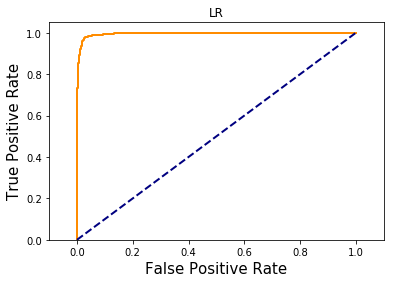
\includegraphics{Figures/LR_1.png}}
\caption{ROC curve of logistic classifier without regularization}
\label{fig:LR1}
\end{figure}

\begin{table}[h]
\center
\caption{Classification quanlity of logistic regression without regularization}
\scalebox{0.9}{
\begin{tabular}{r|c}
\hline
Confusion Matrix & [1500 60 ; 32 1558] \\\hline
Accuracy & 0.9708 \\\hline
Recall & 0.9799 \\\hline
Precision & 0.9629 \\\hline
F1 Score & 0.9713\\\hline
\end{tabular}}
\label{tab:LR1}
\end{table}

Now by applying 5-fold cross-validation on the training data just like previously discussed, we found that the best regularization strength is $10$ for L1 regularization and $100$ for l2 regularization. The ROC curve of those logistic classifiers with regularization are shown in Figure \ref {fig:LR2} and Figure \ref{fig:LR3}. The other classification measure results are presented in Table \ref{tab:LR2} and Table \ref{tab:LR3}.

\bigbreak

By comparing the performance results of those three logistic classifiers: without regularization, with L1 regularization and L2 regularization, we can conclude that the logistic classifier with L2 regularization does the best job.

\bigbreak

Like Owen Zheng said, if you are using regression without regularization, you have to be very special. Technically speaking, regularization would constrain learning a way more complex model, so as to avoid the risk of overfitting. In term of coefficient,  regularization is kind of a form of regression that would shrink the coefficient estimates towards zero. That's why adding regularization would facilitate generalization ability of the classifier and improve the performance when applying test data. For example, if there is noise in the training data, then the estimated coefficients won't generalize well to the future test data. This is where regularization comes in and regularizes these learned estimates towards zero. However it's also a trade off to choose a great and appropriate regularization strength. Increasing regularization parameter results in less overfitting bus also greater bias, which still would decrease the performance of the classifier.

\bigbreak

When it comes to choosing a type of regularization, the differences of L1-norm and L2-norm as a loss function can be promptly summarized as Table \ref{tab:L1L2}. Intuitively, the key difference between these two regularization methods is that L1 can be used for noisy data, which is very appealing and on the other hand L2 has a closed form solution in an optimization setting.

\bigbreak

Even though logistic regression and linear SVM both are using a linear decision boundary, the concept or motivation behind the algorithm is totally different. Logistic regression focuses on maximizing the probability of the data. The farther the data lies from the separating hyperplane on the correct side, the happier it is. On the other hand, an SVM just tries to find the hyperplane that maximizes the distance of the closet points to the margin. If a point is not a support vector, it doesn't really matter. Therefore, depending on the problem and data, their performance would differ.

\begin{table}[h]
\center
\caption{Comparison between L1 and L2 regularization}
\scalebox{0.9}{
\begin{tabular}{l|c|c}
\hline
& L1 regularization & L2 regularization\\\hline
Robustness & robust & not very robust \\\hline
Stability & unstable solution & stable solution \\\hline
Uniqueness & possibly multiple solutions & always one solution \\\hline
\end{tabular}}
\label{tab:L1L2}
\end{table}



\begin{figure}[h]
\centering
\scalebox{0.9}{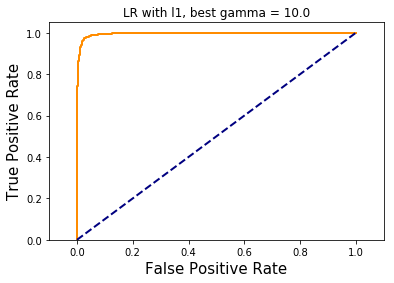
\includegraphics{Figures/LR_2.png}}
\caption{ROC curve of logistic classifier with regularization L1}
\label{fig:LR2}
\end{figure}

\begin{table}[h]
\center
\caption{Classification quanlity of logistic regression with regularization L1}
\scalebox{0.9}{
\begin{tabular}{r|c}
\hline
Confusion Matrix & [1501 59 ; 33 1557] \\\hline
Accuracy & 0.9708 \\\hline
Recall & 0.9792 \\\hline
Precision & 0.9635 \\\hline
F1 Score & 0.9713\\\hline
\end{tabular}}
\label{tab:LR2}
\end{table}

\begin{figure}[h]
\centering
\scalebox{0.9}{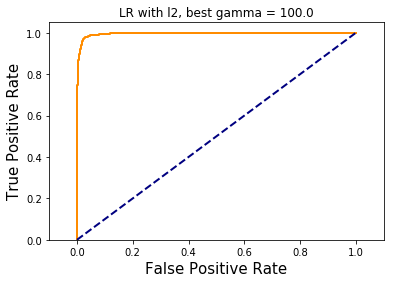
\includegraphics{Figures/LR_3.png}}
\caption{ROC curve of logistic classifier with regularization L2}
\label{fig:LR3}
\end{figure}

\begin{table}[h]
\center
\caption{Classification quanlity of logistic regression with regularization L2}
\scalebox{0.9}{
\begin{tabular}{r|c}
\hline
Confusion Matrix & [1505 66 ; 30 1560] \\\hline
Accuracy & 0.9727 \\\hline
Recall & 0.9911 \\\hline
Precision & 0.9653 \\\hline
F1 Score & 0.9732\\\hline
\end{tabular}}
\label{tab:LR3}
\end{table}

\subsubsection{Naive Bayes}

\textbf{Question 6:}

This time, we trained a naive Bayes classifier. The ROC curve is shown in Figure \ref {fig:By1}. The other classification measure results are presented in Table \ref{tab:By1}.

\bigbreak

\begin{figure}[h]
\centering
\scalebox{0.9}{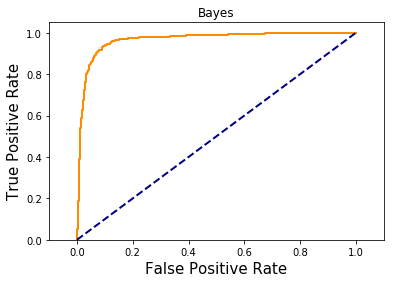
\includegraphics{Figures/Bayes.png}}
\caption{ROC curve of naive Bayes classifier}
\label{fig:By1}
\end{figure}

\begin{table}[h]
\center
\caption{Classification quanlity of naive Bayes classifier}
\scalebox{0.9}{
\begin{tabular}{r|c}
\hline
Confusion Matrix & [1334 226 ; 56 1534] \\\hline
Accuracy & 0.9105 \\\hline
Recall & 0.9648 \\\hline
Precision & 0.8716 \\\hline
F1 Score & 0.9158\\\hline
\end{tabular}}
\label{tab:By1}
\end{table}

\subsubsection{Grid Search of Parameters}

\textbf{Question 7:}

We do grid search with 5-fold cross-validation for different classifiers with different parameters and compare their test accuracy. The results of removing "headers" and "footers" are shown in Table \ref{tab:By0} and the results of not removing "headers" and "footers" are shown in Table \ref{tab:By2}. Due to the width of the table, it can't be shown completely. The complete table is in the excel document named "q7".

\bigbreak

From the two tables, we can get the following analysis: Min\_df does not have much influence on mean\_test\_score, because the mean\_test\_scores when we choose Min\_df=3 or Min\_df=5 are very close. Lemmatization has much influence on mean\_test\_score. Mean\_test\_score improves significantly when we use lemmatization than not. In most cases, mean\_test\_score is higher when we use LSI to reduce dimensionality than using NMF. But if we choose GaussianNB classifier and use lemmatization, NMF is better than LSI. As for different classifiers, the performance of GaussianNB is the worst and the performance of the other three classifiers is very close. And the performance improves a little when we do not remove “headers” and “footers” than we do. 

\bigbreak

The best combination is this: The classifier is SVM or Logistic Regression with L1 or L2 regularization(because their performances are really close to each other). Do not remove “headers” and “footers”. Use lemmatization. Use LSI to do dimensionality reduction.
And min\_df=3(But in some cases min\_df=5 has better performance).

\bigbreak

\begin{table}[h]
\center
\caption{Removing "headers" and "footers"}
\scalebox{0.9}{
\begin{tabular}{r|c|c|c|c|c|c|c|c|c|c|c|c|c|c|c|c|c|c|c|c|c}
\hline
 & param clf & param clf  C & param reduce dim & param vect  analyzer & param vect  min df & mean test score & rank test score & split0 train score & split1 train score & split2 train score & split3 train score & split4 train score & mean train score & std train score\\\hline
0 & LinearSVC & 10 & TruncatedSVD(algorithm='randomized', n compone... & <function stem rmv punc at 0x000001CE84CF4EA0> & 3 & 0.967033 & 5 & 0.972259 & 0.969881 & 0.971731 & 0.971738 & 0.975706 & 0.972263 & 0.001902\\\hline
1 & LinearSVC & 10 & TruncatedSVD(algorithm='randomized', n compone... & <function stem rmv punc at 0x000001CE84CF4EA0> & 5 & 0.968301 & 3 & 0.973316 & 0.969353 & 0.973844 & 0.973323 & 0.967785 & 0.971524 & 0.002471\\\hline
2 & LinearSVC & 10 & TruncatedSVD(algorithm='randomized', n compone... & <function dumb stem at 0x000001CE84D11598> & 3 & 0.801564 & 17 & 0.799736 & 0.801585 & 0.802642 & 0.806392 & 0.806443 & 0.80336 & 0.002665\\\hline
3 & LinearSVC & 10 & TruncatedSVD(algorithm='randomized', n compone... & <function dumb stem at 0x000001CE84D11598> & 5 & 0.801564 & 17 & 0.799472 & 0.801585 & 0.802642 & 0.806128 & 0.805651 & 0.803096 & 0.002504\\\hline
4 & LinearSVC & 10 & NMF(alpha=0.0, beta loss='frobenius', init=Non... & <function stem rmv punc at 0x000001CE84CF4EA0> & 3 & 0.959848 & 10 & 0.961427 & 0.957464 & 0.95852 & 0.961701 & 0.960655 & 0.959953 & 0.001671\\\hline
5 & LinearSVC & 10 & NMF(alpha=0.0, beta loss='frobenius', init=Non... & <function stem rmv punc at 0x000001CE84CF4EA0> & 5 & 0.958791 & 12 & 0.959313 & 0.957992 & 0.963804 & 0.962229 & 0.961183 & 0.960904 & 0.002062\\\hline
6 & LinearSVC & 10 & NMF(alpha=0.0, beta loss='frobenius', init=Non... & <function dumb stem at 0x000001CE84D11598> & 3 & 0.784235 & 25 & 0.794716 & 0.786262 & 0.793923 & 0.788959 & 0.800898 & 0.792952 & 0.005058\\\hline
7 & LinearSVC & 10 & NMF(alpha=0.0, beta loss='frobenius', init=Non... & <function dumb stem at 0x000001CE84D11598> & 5 & 0.782544 & 28 & 0.794716 & 0.786262 & 0.793923 & 0.782884 & 0.799313 & 0.79142 & 0.005982\\\hline
8 & GaussianNB & NaN & TruncatedSVD(algorithm='randomized', n compone... & <function stem rmv punc at 0x000001CE84CF4EA0> & 3 & 0.843407 & 15 & 0.868956 & 0.84148 & 0.858388 & 0.859218 & 0.865329 & 0.858674 & 0.009445\\\hline
9 & GaussianNB & NaN & TruncatedSVD(algorithm='randomized', n compone... & <function stem rmv punc at 0x000001CE84CF4EA0> & 5 & 0.839814 & 16 & 0.861295 & 0.84465 & 0.85469 & 0.85552 & 0.861368 & 0.855504 & 0.006106\\\hline
10 & GaussianNB & NaN & TruncatedSVD(algorithm='randomized', n compone... & <function dumb stem at 0x000001CE84D11598> & 3 & 0.6306 & 29 & 0.591546 & 0.612153 & 0.67926 & 0.633122 & 0.641669 & 0.63155 & 0.029522\\\hline
11 & GaussianNB & NaN & TruncatedSVD(algorithm='randomized', n compone... & <function dumb stem at 0x000001CE84D11598> & 5 & 0.629966 & 30 & 0.591546 & 0.612153 & 0.67926 & 0.635763 & 0.640349 & 0.631814 & 0.029488\\\hline
12 & GaussianNB & NaN & NMF(alpha=0.0, beta loss='frobenius', init=Non... & <function stem rmv punc at 0x000001CE84CF4EA0> & 3 & 0.94104 & 14 & 0.94716 & 0.941347 & 0.941876 & 0.943476 & 0.941378 & 0.943047 & 0.002197\\\hline
13 & GaussianNB & NaN & NMF(alpha=0.0, beta loss='frobenius', init=Non... & <function stem rmv punc at 0x000001CE84CF4EA0> & 5 & 0.942308 & 13 & 0.949273 & 0.937384 & 0.947424 & 0.942948 & 0.94085 & 0.943576 & 0.004323\\\hline
14 & GaussianNB & NaN & NMF(alpha=0.0, beta loss='frobenius', init=Non... & <function dumb stem at 0x000001CE84D11598> & 3 & 0.606932 & 31 & 0.604227 & 0.611625 & 0.635931 & 0.615689 & 0.613414 & 0.616177 & 0.010598\\\hline
15 & GaussianNB & NaN & NMF(alpha=0.0, beta loss='frobenius', init=Non... & <function dumb stem at 0x000001CE84D11598> & 5 & 0.606298 & 32 & 0.604227 & 0.611625 & 0.635931 & 0.619123 & 0.615263 & 0.617234 & 0.010561\\\hline
16 & LogisticRegression & 10 & TruncatedSVD(algorithm='randomized', n compone... & <function stem rmv punc at 0x000001CE84CF4EA0> & 3 & 0.967878 & 4 & 0.973844 & 0.972523 & 0.97358 & 0.973059 & 0.974122 & 0.973426 & 0.000572\\\hline
17 & LogisticRegression & 10 & TruncatedSVD(algorithm='randomized', n compone... & <function stem rmv punc at 0x000001CE84CF4EA0> & 5 & 0.968724 & 2 & 0.974373 & 0.97041 & 0.974373 & 0.973323 & 0.971217 & 0.972739 & 0.001638\\\hline
18 & LogisticRegression & 10 & TruncatedSVD(algorithm='randomized', n compone... & <function dumb stem at 0x000001CE84D11598> & 3 & 0.80093 & 20 & 0.800264 & 0.802114 & 0.800793 & 0.809033 & 0.806707 & 0.803782 & 0.003471\\\hline
19 & LogisticRegression & 10 & TruncatedSVD(algorithm='randomized', n compone... & <function dumb stem at 0x000001CE84D11598> & 5 & 0.801564 & 17 & 0.800264 & 0.802114 & 0.800793 & 0.808241 & 0.807499 & 0.803782 & 0.0034\\\hline
20 & LogisticRegression & 10 & NMF(alpha=0.0, beta loss='frobenius', init=Non... & <function stem rmv punc at 0x000001CE84CF4EA0> & 3 & 0.963018 & 8 & 0.966975 & 0.963276 & 0.966711 & 0.964871 & 0.964616 & 0.96529 & 0.001382\\\hline
21 & LogisticRegression & 10 & NMF(alpha=0.0, beta loss='frobenius', init=Non... & <function stem rmv punc at 0x000001CE84CF4EA0> & 5 & 0.963863 & 7 & 0.964069 & 0.964333 & 0.969089 & 0.966455 & 0.96752 & 0.966293 & 0.001905\\\hline
22 & LogisticRegression & 10 & NMF(alpha=0.0, beta loss='frobenius', init=Non... & <function dumb stem at 0x000001CE84D11598> & 3 & 0.78508 & 24 & 0.797886 & 0.796301 & 0.794452 & 0.789223 & 0.799578 & 0.795488 & 0.003562\\\hline
23 & LogisticRegression & 10 & NMF(alpha=0.0, beta loss='frobenius', init=Non... & <function dumb stem at 0x000001CE84D11598> & 5 & 0.785292 & 23 & 0.797886 & 0.796301 & 0.794452 & 0.789223 & 0.798785 & 0.79533 & 0.003391\\\hline
24 & LogisticRegression & 100 & TruncatedSVD(algorithm='randomized', n compone... & <function stem rmv punc at 0x000001CE84CF4EA0> & 3 & 0.967033 & 5 & 0.974637 & 0.971202 & 0.972787 & 0.972795 & 0.975706 & 0.973425 & 0.001576\\\hline
25 & LogisticRegression & 100 & TruncatedSVD(algorithm='randomized', n compone... & <function stem rmv punc at 0x000001CE84CF4EA0> & 5 & 0.968935 & 1 & 0.973052 & 0.970674 & 0.975958 & 0.973323 & 0.971217 & 0.972845 & 0.001861\\\hline
26 & LogisticRegression & 100 & TruncatedSVD(algorithm='randomized', n compone... & <function dumb stem at 0x000001CE84D11598> & 3 & 0.800507 & 22 & 0.799736 & 0.802378 & 0.801585 & 0.81009 & 0.806179 & 0.803994 & 0.003701\\\hline
27 & LogisticRegression & 100 & TruncatedSVD(algorithm='randomized', n compone... & <function dumb stem at 0x000001CE84D11598> & 5 & 0.800719 & 21 & 0.799736 & 0.802378 & 0.801585 & 0.807977 & 0.808556 & 0.804046 & 0.003555\\\hline
28 & LogisticRegression & 100 & NMF(alpha=0.0, beta loss='frobenius', init=Non... & <function stem rmv punc at 0x000001CE84CF4EA0> & 3 & 0.960059 & 9 & 0.961955 & 0.957199 & 0.959313 & 0.963022 & 0.961447 & 0.960587 & 0.00208\\\hline
29 & LogisticRegression & 100 & NMF(alpha=0.0, beta loss='frobenius', init=Non... & <function stem rmv punc at 0x000001CE84CF4EA0> & 5 & 0.959848 & 10 & 0.96037 & 0.959049 & 0.965125 & 0.963814 & 0.963824 & 0.962436 & 0.002315\\\hline
30 & LogisticRegression & 100 & NMF(alpha=0.0, beta loss='frobenius', init=Non... & <function dumb stem at 0x000001CE84D11598> & 3 & 0.784024 & 26 & 0.793923 & 0.787054 & 0.795244 & 0.790016 & 0.799842 & 0.793216 & 0.004398\\\hline
31 & LogisticRegression & 100 & NMF(alpha=0.0, beta loss='frobenius', init=Non... & <function dumb stem at 0x000001CE84D11598> & 5 & 0.782756 & 27 & 0.793923 & 0.787054 & 0.795244 & 0.784997 & 0.80037 & 0.792318 & 0.005608\\\hline





\end{tabular}}
\label{tab:By0}
\end{table}

\begin{table}[h]
\center
\caption{Not removing "headers" and "footers"}
\scalebox{0.9}{
\begin{tabular}{r|c|c|c|c|c|c|c|c|c|c|c|c|c|c|c|c|c|c|c|c|c}
\hline
 & param clf & param clf  C & param reduce dim & param vect  analyzer & param vect  min df & mean test score & rank test score & split0 train score & split1 train score & split2 train score & split3 train score & split4 train score & mean train score & std train score\\\hline
0 & LinearSVC & 10 & TruncatedSVD(algorithm='randomized', n compone... & <function stem rmv punc at 0x0000022A20CAAF28> & 3 & 0.97612 & 2 & 0.980185 & 0.977279 & 0.977543 & 0.980983 & 0.978611 & 0.97892 & 0.001452\\\hline
1 & LinearSVC & 10 & TruncatedSVD(algorithm='randomized', n compone... & <function stem rmv punc at 0x0000022A20CAAF28> & 5 & 0.974218 & 6 & 0.977543 & 0.977543 & 0.978336 & 0.979662 & 0.978083 & 0.978233 & 0.000778\\\hline
2 & LinearSVC & 10 & TruncatedSVD(algorithm='randomized', n compone... & <function dumb stem at 0x0000022A20CC5620> & 3 & 0.780642 & 20 & 0.790489 & 0.782299 & 0.782299 & 0.798996 & 0.793768 & 0.78957 & 0.006528\\\hline
3 & LinearSVC & 10 & TruncatedSVD(algorithm='randomized', n compone... & <function dumb stem at 0x0000022A20CC5620> & 5 & 0.782544 & 17 & 0.791017 & 0.780449 & 0.781242 & 0.798996 & 0.792712 & 0.788883 & 0.007085\\\hline
4 & LinearSVC & 10 & NMF(alpha=0.0, beta loss='frobenius', init=Non... & <function stem rmv punc at 0x0000022A20CAAF28> & 3 & 0.96809 & 9 & 0.966182 & 0.967503 & 0.964861 & 0.966191 & 0.9662 & 0.966188 & 0.000836\\\hline
5 & LinearSVC & 10 & NMF(alpha=0.0, beta loss='frobenius', init=Non... & <function stem rmv punc at 0x0000022A20CAAF28> & 5 & 0.96809 & 9 & 0.965125 & 0.968032 & 0.966711 & 0.96804 & 0.965408 & 0.966663 & 0.001242\\\hline
6 & LinearSVC & 10 & NMF(alpha=0.0, beta loss='frobenius', init=Non... & <function dumb stem at 0x0000022A20CC5620> & 3 & 0.76585 & 27 & 0.765125 & 0.76539 & 0.767768 & 0.775489 & 0.767626 & 0.768279 & 0.003767\\\hline
7 & LinearSVC & 10 & NMF(alpha=0.0, beta loss='frobenius', init=Non... & <function dumb stem at 0x0000022A20CC5620> & 5 & 0.767963 & 26 & 0.766446 & 0.766975 & 0.769617 & 0.777073 & 0.77502 & 0.771026 & 0.004287\\\hline
8 & GaussianNB & NaN & TruncatedSVD(algorithm='randomized', n compone... & <function stem rmv punc at 0x0000022A20CAAF28> & 3 & 0.905325 & 15 & 0.919947 & 0.917834 & 0.890621 & 0.880877 & 0.925799 & 0.907015 & 0.017827\\\hline
9 & GaussianNB & NaN & TruncatedSVD(algorithm='randomized', n compone... & <function stem rmv punc at 0x0000022A20CAAF28> & 5 & 0.898986 & 16 & 0.929987 & 0.899075 & 0.883752 & 0.884575 & 0.924478 & 0.904373 & 0.019522\\\hline
10 & GaussianNB & NaN & TruncatedSVD(algorithm='randomized', n compone... & <function dumb stem at 0x0000022A20CC5620> & 3 & 0.640744 & 30 & 0.633554 & 0.636196 & 0.642801 & 0.638933 & 0.658041 & 0.641905 & 0.008629\\\hline
11 & GaussianNB & NaN & TruncatedSVD(algorithm='randomized', n compone... & <function dumb stem at 0x0000022A20CC5620> & 5 & 0.641589 & 29 & 0.634875 & 0.63461 & 0.644122 & 0.637612 & 0.660417 & 0.642327 & 0.009673\\\hline
12 & GaussianNB & NaN & NMF(alpha=0.0, beta loss='frobenius', init=Non... & <function stem rmv punc at 0x0000022A20CAAF28> & 3 & 0.945266 & 13 & 0.944782 & 0.942933 & 0.943461 & 0.945325 & 0.947452 & 0.94479 & 0.001587\\\hline
13 & GaussianNB & NaN & NMF(alpha=0.0, beta loss='frobenius', init=Non... & <function stem rmv punc at 0x0000022A20CAAF28> & 5 & 0.943787 & 14 & 0.945046 & 0.950066 & 0.945575 & 0.941363 & 0.944811 & 0.945372 & 0.002777\\\hline
14 & GaussianNB & NaN & NMF(alpha=0.0, beta loss='frobenius', init=Non... & <function dumb stem at 0x0000022A20CC5620> & 3 & 0.61623 & 31 & 0.606869 & 0.612946 & 0.628005 & 0.605388 & 0.647742 & 0.62019 & 0.015932\\\hline
15 & GaussianNB & NaN & NMF(alpha=0.0, beta loss='frobenius', init=Non... & <function dumb stem at 0x0000022A20CC5620> & 5 & 0.615173 & 32 & 0.608719 & 0.614531 & 0.638309 & 0.606973 & 0.642461 & 0.622199 & 0.015116\\\hline
16 & LogisticRegression & 10 & TruncatedSVD(algorithm='randomized', n compone... & <function stem rmv punc at 0x0000022A20CAAF28> & 3 & 0.976965 & 1 & 0.978864 & 0.9786 & 0.977807 & 0.980983 & 0.979403 & 0.979131 & 0.001059\\\hline
17 & LogisticRegression & 10 & TruncatedSVD(algorithm='randomized', n compone... & <function stem rmv punc at 0x0000022A20CAAF28> & 5 & 0.974852 & 4 & 0.977807 & 0.979392 & 0.9786 & 0.978077 & 0.978611 & 0.978497 & 0.000544\\\hline
18 & LogisticRegression & 10 & TruncatedSVD(algorithm='randomized', n compone... & <function dumb stem at 0x0000022A20CC5620> & 3 & 0.780642 & 20 & 0.793131 & 0.782563 & 0.784676 & 0.798732 & 0.790599 & 0.78994 & 0.005832\\\hline
19 & LogisticRegression & 10 & TruncatedSVD(algorithm='randomized', n compone... & <function dumb stem at 0x0000022A20CC5620> & 5 & 0.780008 & 22 & 0.791281 & 0.782827 & 0.783091 & 0.798204 & 0.792448 & 0.78957 & 0.005886\\\hline
20 & LogisticRegression & 10 & NMF(alpha=0.0, beta loss='frobenius', init=Non... & <function stem rmv punc at 0x0000022A20CAAF28> & 3 & 0.972316 & 7 & 0.969353 & 0.969881 & 0.970938 & 0.971474 & 0.970689 & 0.970467 & 0.000758\\\hline
21 & LogisticRegression & 10 & NMF(alpha=0.0, beta loss='frobenius', init=Non... & <function stem rmv punc at 0x0000022A20CAAF28> & 5 & 0.969358 & 8 & 0.971466 & 0.967768 & 0.970938 & 0.972002 & 0.97201 & 0.970837 & 0.001585\\\hline
22 & LogisticRegression & 10 & NMF(alpha=0.0, beta loss='frobenius', init=Non... & <function dumb stem at 0x0000022A20CC5620> & 3 & 0.771555 & 24 & 0.778336 & 0.769353 & 0.769089 & 0.783148 & 0.775548 & 0.775095 & 0.005378\\\hline
23 & LogisticRegression & 10 & NMF(alpha=0.0, beta loss='frobenius', init=Non... & <function dumb stem at 0x0000022A20CC5620> & 5 & 0.774091 & 23 & 0.777543 & 0.769089 & 0.779392 & 0.789752 & 0.781093 & 0.779374 & 0.00663\\\hline
24 & LogisticRegression & 100 & TruncatedSVD(algorithm='randomized', n compone... & <function stem rmv punc at 0x0000022A20CAAF28> & 3 & 0.975697 & 3 & 0.979128 & 0.977279 & 0.977543 & 0.980983 & 0.978875 & 0.978761 & 0.001324\\\hline
25 & LogisticRegression & 100 & TruncatedSVD(algorithm='randomized', n compone... & <function stem rmv punc at 0x0000022A20CAAF28> & 5 & 0.974429 & 5 & 0.977015 & 0.977543 & 0.978336 & 0.979398 & 0.978611 & 0.97818 & 0.000832\\\hline
26 & LogisticRegression & 100 & TruncatedSVD(algorithm='randomized', n compone... & <function dumb stem at 0x0000022A20CC5620> & 3 & 0.781065 & 19 & 0.792867 & 0.78362 & 0.785205 & 0.799525 & 0.79324 & 0.790891 & 0.005817\\\hline
27 & LogisticRegression & 100 & TruncatedSVD(algorithm='randomized', n compone... & <function dumb stem at 0x0000022A20CC5620> & 5 & 0.782544 & 17 & 0.792867 & 0.781506 & 0.782563 & 0.799525 & 0.79192 & 0.789676 & 0.006776\\\hline
28 & LogisticRegression & 100 & NMF(alpha=0.0, beta loss='frobenius', init=Non... & <function stem rmv punc at 0x0000022A20CAAF28> & 3 & 0.967033 & 11 & 0.963804 & 0.966975 & 0.964861 & 0.966455 & 0.965408 & 0.965501 & 0.00113\\\hline
29 & LogisticRegression & 100 & NMF(alpha=0.0, beta loss='frobenius', init=Non... & <function stem rmv punc at 0x0000022A20CAAF28> & 5 & 0.966399 & 12 & 0.964861 & 0.967503 & 0.966182 & 0.967248 & 0.964616 & 0.966082 & 0.001186\\\hline
30 & LogisticRegression & 100 & NMF(alpha=0.0, beta loss='frobenius', init=Non... & <function dumb stem at 0x0000022A20CC5620> & 3 & 0.763736 & 28 & 0.768032 & 0.765125 & 0.768032 & 0.77496 & 0.768154 & 0.768861 & 0.003257\\\hline
31 & LogisticRegression & 100 & NMF(alpha=0.0, beta loss='frobenius', init=Non... & <function dumb stem at 0x0000022A20CC5620> & 5 & 0.769231 & 25 & 0.767768 & 0.767768 & 0.770145 & 0.777602 & 0.778189 & 0.772294 & 0.004659\\\hline






\end{tabular}}
\label{tab:By2}
\end{table}



\section{Multiclass Classification}

\textbf{Question 8:}

The results of different multiclass classification are shown in Table \ref{tab:By3},Table \ref{tab:By4},Table \ref{tab:By5},Table \ref{tab:By6},Table \ref{tab:By7},Table \ref{tab:By8}.

\bigbreak

From the results, we can get the following conclusions: For multiclass classification task, SVM has better performance than Naïve Bayes. And OneVsOne SVM and OneVsRest SVM have similar classification performances. As for dimension reduction methods in this question, LSI has better performance than NMF when we use SVM, but has worse performance than NMF when we use Naïve Bayes.

\begin{table}[h]
\center
\caption{Use LSI to reduce dimension, GaussianNB classification}
\scalebox{0.9}{
\begin{tabular}{r|c}
\hline
Confusion Matrix & [[226  42 122   2]\\
 & [107 148 128   2]\\
 & [ 43  47 298   2]\\
 & [  0   1  15 382]]
 \\\hline
Accuracy & 0.6735 \\\hline
Recall & 0.6735 \\\hline
Precision & 0.6858 \\\hline
F1 Score & 0.6673\\\hline
\end{tabular}}
\label{tab:By3}
\end{table}

\begin{table}[h]
\center
\caption{Use LSI to reduce dimension, OneVsOneSVM classification}
\scalebox{0.9}{
\begin{tabular}{r|c}
\hline
Confusion Matrix & [[330  40  22   0]\\&
 [ 42 322  21   0]\\&
 [ 26  20 343   1]\\&
 [  5   1   4 388]]
 \\\hline
Accuracy & 0.8837 \\\hline
Recall & 0.8837 \\\hline
Precision & 0.8848 \\\hline
F1 Score & 0.8842\\\hline
\end{tabular}}
\label{tab:By4}
\end{table}

\begin{table}[h]
\center
\caption{Use LSI to reduce dimension, OneVsRestSVM classification}
\scalebox{0.9}{
\begin{tabular}{r|c}
\hline
Confusion Matrix & [[317  47  26   2]\\&
 [ 34 330  20   1]\\&
 [ 17  21 348   4]\\&
 [  2   0   2 394]]
 \\\hline
Accuracy & 0.8875 \\\hline
Recall & 0.8875 \\\hline
Precision & 0.8874 \\\hline
F1 Score & 0.8872\\\hline
\end{tabular}}
\label{tab:By5}
\end{table}

\begin{table}[h]
\center
\caption{Use NMF to reduce dimension, GaussianNB classification}
\scalebox{0.9}{
\begin{tabular}{r|c}
\hline
Confusion Matrix & [[275  53  56   8]\\&
 [116 221  44   4]\\&
 [ 48  36 290  16]\\&
 [  1   1   5 391]]
 \\\hline
Accuracy & 0.7521 \\\hline
Recall & 0.7521 \\\hline
Precision & 0.7516 \\\hline
F1 Score & 0.7494\\\hline
\end{tabular}}
\label{tab:By6}
\end{table}

\begin{table}[h]
\center
\caption{Use NMF to reduce dimension, OneVsOneSVM classification}
\scalebox{0.9}{
\begin{tabular}{r|c}
\hline
Confusion Matrix & [[303  62  27   0]\\&
 [ 70 291  23   1]\\&
 [ 37  14 337   2]\\&
 [  4   1   4 389]]
 \\\hline
Accuracy & 0.8435 \\\hline
Recall & 0.8435 \\\hline
Precision & 0.8450 \\\hline
F1 Score & 0.8440\\\hline
\end{tabular}}
\label{tab:By7}
\end{table}

\begin{table}[h]
\center
\caption{Use NMF to reduce dimension, OneVsRestSVM classification}
\scalebox{0.9}{
\begin{tabular}{r|c}
\hline
Confusion Matrix & [[294  70  28   0]\\&
 [ 66 293  22   4]\\&
 [ 33  15 338   4]\\&
 [  3   2   2 391]]
 \\\hline
Accuracy & 0.8409 \\\hline
Recall & 0.8409 \\\hline
Precision & 0.8408 \\\hline
F1 Score & 0.8409\\\hline
\end{tabular}}
\label{tab:By8}
\end{table}


\end{document}
